\documentclass[12pt, twoside]{article}
%\usepackage[hmargin=1.25in, vmargin=1.1in]{geometry}
\usepackage{geometry}

\usepackage[utf8]{inputenc}
\usepackage[T1]{fontenc}
\usepackage[english]{babel}
\usepackage{pdfpages}
\usepackage{listings}
\usepackage{color}
\usepackage{graphicx}
\usepackage{float}
\usepackage{hyperref}
\usepackage{url}
\usepackage{upquote}
\usepackage{lastpage}
\usepackage{fancyhdr}
\pagestyle{fancy}
\usepackage{longtable}
\usepackage{tabu}
\usepackage{rotating}
\usepackage[strings]{underscore}
\usepackage[nottoc,numbib]{tocbibind}
\usepackage{float}
\restylefloat{table}

\graphicspath{ {images/} }

\newcommand{\helv}{\fontfamily{phv}\fontseries{b}\fontsize{9}{11}\selectfont}

%--------------- Variables à modifier à chaque rendu ---------------
\title{Report}
\newcommand{\daterendu}{09/08/2019}
%-------------------------------------------------------------------

\makeatletter\let\Title\@title\makeatother

% Décommenter pour commencer les chapitres à 0
%\setcounter{section}{-1}

\begin{document}

\begin{titlepage}

\newcommand{\HRule}{\rule{\linewidth}{0.5mm}} % Defines a new command for the horizontal lines, change thickness here

\center % Center everything on the page



\includegraphics[width=0.8\textwidth]{logo_HEIA.jpg}

\includegraphics[width=0.3\textwidth]{logo_LBNL.png}\\[1.1cm]
\textsc{\Large Bachelor thesis \\ [0.3cm]
\large Year 2018-2019 }\\ [2.0cm]


\textsc{
\bfseries \LARGE Machine learning for noise reduction in images of old audio records}\\ [1.0cm]


\HRule \\[0.5cm]
{ \huge \bfseries \Title }\\ 
\HRule \\[1.2cm]

\Large
Benoit \textsc{Ruffray}\\[1.0cm] 

{\large Date : \daterendu}\\[1.3cm] 

\begin{flushleft}
\large External supervisor: Haber~Carl
\end{flushleft}
\begin{flushleft}
	\large Internal supervisors: Bapst~Frédéric / Hennebert~Jean
\end{flushleft}
\begin{flushleft}
\large Consultants: Cornell~Earl / Nachman~Benjamin
\end{flushleft}

\end{titlepage}
\pagenumbering{Roman}

\renewcommand{\headrulewidth}{1pt}
\fancyhead[L]{\helv ML-for-NR}
\fancyhead[C]{\helv 2018-2019}
\fancyhead[R]{\helv \Title }

\renewcommand{\footrulewidth}{1pt}
\fancyfoot[C]{\helv Table of contents \thepage{}}

\setcounter{page}{1}

\begin{center}
\tableofcontents
\end{center}

\newpage

\fancyhf{}
\renewcommand{\headrulewidth}{1pt}
\fancyhead[L]{\helv ML-for-NR}
\fancyhead[C]{\helv 2018-2019}
\fancyhead[R]{\helv \Title }

\renewcommand{\footrulewidth}{1pt}
\fancyfoot[LO, RE]{\helv Bachelor thesis, year 2018 - 2019}
\fancyfoot[C]{}
\fancyfoot[RO, LE]{\helv \textbf{Page \thepage{}/\pageref{LastPage}}}
\pagenumbering{arabic}
\setcounter{page}{1}
\begin{abstract}
	Sample text.
\end{abstract}
\renewcommand{\abstractname}{Acknowledgements}
\begin{abstract}
	Sample text.
\end{abstract}

\section{Introduction}
This document is the final report of the Bachelor project "Machine learning for noise reduction in images of old audio records". It contains all information regarding the project, from the context to the details of implementation. This project is done under the supervision of Mr. Carl Haber at the Lawrence Berkeley National Laboratory, and supervised by Messrs. Frédéric Bapst and Jean Hennebert at the University of Applied Science of Fribourg.

"Machine learning for noise reduction in images of old audio records" (ML4NR) is a project proposed by Mr. Carl Haber at the Lawrence Berkeley National Laboratory (LBNL). It is part of a project for the Library of Congress, whose goal is the restoration and preservation of old audio records.
ML4NR is done as a Bachelor Thesis project by Mr. Benoît Ruffray
\subsection{Report organization}
This report starts with an explanation of the context regarding audio records, IRENE/Weaver, and machine learning. It continues by detailing the objectives of the project and the tasks planning. Then, each major step is explained in its own section, from the analysis to the testing. Finally, the conclusion and personal review resumes it all.
\subsection{Folder organization}
The project folder contains a \texttt{doc} folder and a \texttt{README} file. The \texttt{doc} folder contains the following elements:
\begin{description}
	\item[data] This folder contains everything regarding the properties of the data used and the system's architecture.
	\item[images] This folder contains the images used for the different documents.
	\item[planning] This folder contains the files used for Gantt planning.
	\item[pv] This folder contains all the meeting minutes.
	\item[report] This folder contains the report document.
	\item[specifications] This folder contains the specification document.
\end{description}
%add folder for keras code
The code developed for Weaver is only available on its GitHub repository. The disc images and music can be found in the Google Drive folder, as they take a lot of space.
\section{Context}
\subsection{Mechanical Audio records}
The first device able to record and play back sound waves was an invention of Thomas Edison in 1877, the cylinder phonograph\cite{audio}. This device could record sounds by making a needle vibrate and carve a groove on a rotating tinfoil or wax cylinder. To play it back, the cylinder was rotated, making the needle vibrate while following the groove. This vibration is amplified and produces audible sound waves, the ones recorded.

Since cylinders were impractical to store and quick to be damaged (the physical contact would wear the groove out during each play), Emile Berliner improved the concept in 1887 by inventing a flat support for audio recording: discs. Those were easier to stack and reproduce, and therefore quickly overtook the market. The associated reading device is the gramophone.

The standard format from the 1910s to 1950s was a double-sided 78 rpm shellac disc. However, shellac is a brittle material, and the hard needles would wear them out quickly. It's in 1948 that Columbia Records invented the 33 rpm vinyl disc. Vinyl is more expensive but sturdier than shellac, and the longer playtime would compensate for the extra cost. RCA Victor introduced the 45 rpm, smaller vinyl disc, in 1949, effectively cutting the cost by using less material. Both formats replaced the shellac disc.

The Library of Congress is interested in the preservation of these old records, as they contain valuable historical audio data such as presidential speeches, native American interviews, or traditional songs from the past. However, since the cylinders and shellac discs are getting destroyed with each play, they associated with the LBNL to find a way to extract and preserve all data without physical contact (non invasive play back). This collaboration gave birth to IRENE.
\subsection{IRENE}
Stands for Image, Reconstruct, Erase Noise, Etc.
IRENE is a scanning machine used to image discs and cylinders. It's composed of high-resolution 2D/3D cameras and rotating supports for the records.

\begin{figure}[H]
	\centering
	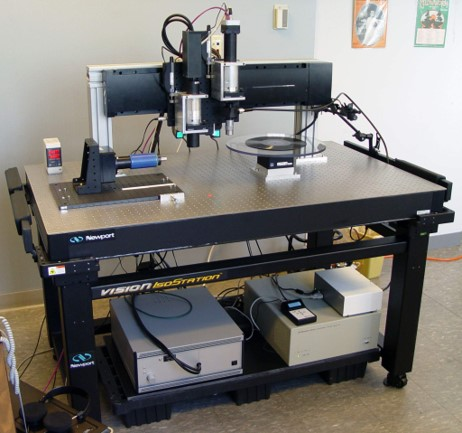
\includegraphics[width=0.5\textwidth]{../images/IRENE.jpg}
	\caption{IRENE (Source : lab's collection)}
	\label{irene}
\end{figure}

The 2D camera takes pictures of one line on the disc, 1 pixel high for thousands of pixels long. The pictures are taken at a very high frequency while the record is turning, imaging the disc line by line. The actual frequency is tuned for the support imaged.

To take pictures, light is directed with a certain angle on the disc. The sensors are activated by the reflected light, and write the perceived amount. Direct reflection results in white pixels, no light reflected becomes black, and in between are the gray scales.
\begin{figure}[H]
	\centering
	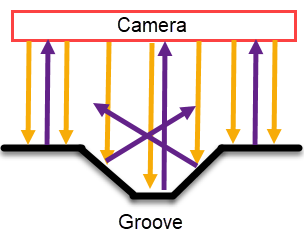
\includegraphics[width=0.5\textwidth]{../images/grooveside.png}
	\caption{Camera lighting the groove and detecting direct reflection (self-made diagram)}
	\label{grooveside}
\end{figure}
The grooves are usually made of large white bands outside (the disc surface), black bands inside (the groove's "walls"), and a thin white in the middle (bottom of the groove). Between these bands, there is a small area of gray scaled pixels.
\begin{figure}[H]
	\centering
	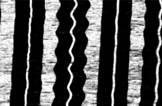
\includegraphics[width=0.5\textwidth]{../images/groove.png}
	\caption{Resulting image of grooves (source : lab's collection)}
	\label{groove}
\end{figure}
Any kind of damage, texture, or unwanted object on the disc can be seen, as it disturbs light reflection. It is considered as noise on the image, and the reason the ML4NR project exists.
\subsection{Weaver}
Along with the IRENE system exists a program named Weaver, made in C\#. It is a collection of plugins developed through the years by researchers and students, used to pipeline the data reading process. 

Weaver's main function is to generate the sound wave from the imaged grooves, using an edge detection algorithm to find the exact center of the groove (figure \ref{edges}). However, since the images are noisy (dust, damage, texture), the sound generated also contains a high frequency background noise. Simply cutting the high frequencies wouldn't completely work, as the noise in images can also influence lower frequencies.

\begin{figure}[H]
	\centering
	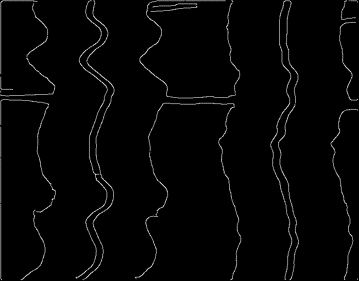
\includegraphics[width=0.5\textwidth]{../images/edges.png}
	\caption{Detected edges. Averaging them gives the center of the groove. (Source : lab's collection)}
	\label{edges}
\end{figure}
\subsection{Machine learning and deep neural networks}
Machine learning is a powerful computing technique used for handling problems having too much parameters for a deterministic algorithm, for example object detection and classification in pictures, or market predictions. It is based on the ability to learn from given correct solutions in order to predict results of future inputs.

Deep neural network is a type of model inspired by the human brain. It is based on multiple layers of neurons. Each neuron takes some data as input, does some transformation, and feeds the output to the next neuron layer. By setting a goal (ground-truth), it can evaluate its result using a loss function, and change slightly the transformations occurring in all layers (weight adjustment). It repeats this process over and over until a threshold is passed.
\subsection{Shellac disc images properties}
This project is aimed at shellac discs, detailed in section \texttt{Mechanical Audio Records}. The LBNL has already imaged a lot of them, and so possesses a consequent collection of groove images.

The shellac discs were imaged at 104 KHz by IRENE, resulting in exactly 80,000 pixels for one revolution. However, those revolutions were divided in 8 parts of 10,000 pixels each. 

IRENE's 2D camera horizontal resolution is 4096 pixels. To obtain a good image quality, it was calibrated to take 3 microns per pixel. This means between 9 and 11 grooves are taken at the same time, and 15 to 30 revolutions are needed to image the entire disc.

So, each shellac disc is imaged with 8 x (15 to 30) pictures of 10,000 x 4096 pixels. All these pictures are in bitmap format and in gray scale.

\begin{figure}
	\centering
	\includegraphics[width=0.4\textwidth]{../images/Vaya-52212c.png}
	\caption{One image of the shellac disc of Vaya Con Dios, by Les Paul and Mary Ford (source : lab's collection)}
	\label{vaya}
\end{figure}
\subsection{Audio data}
For some of the shellac discs, the LBNL possesses the audio source used to press them, coming from a CD or a tape. This gives us a clear reference on what the play back should sounds like. They were typically recorded at 44 KHz.

For the other discs, the audio reconstructed by Weaver can still serve as a good goal for the machine learning model. 

\section{Objectives}
The main goal of the ML4NR project is to generate a cleaner sound than the deterministic algorithm when given noisy groove images as input by using machine learning. It was never attempted before at the LBNL. The project is divided into progressive steps, which correspond to working prototypes.
\subsection{Prototype 0}
This prototype serves as training for using KERAS. It'll teach the basics of model building. Its goal is to have a result on the CIFAR-10 dataset (not necessarily good). 
\subsection{Prototype 1}
This prototype is a proof of concept. Using Weaver, groove images of pure sine waves are generated. They are used to train a model, whose goal will be to find the simple frequency sound wave from the image. A metric needs to be defined for result evaluation.
\subsection{Weaver Plugin}
The previously used Weaver plugin needs to be modified, in order for it to be able to generate noisy groove images. The artificial noise needs to have the same properties as the real one (in actual imaged grooves).
\subsection{Prototype 2}
This prototype tests the robustness of the model built before. It uses the noisy groove images generated with the Weaver plugin as input, and tries to find the clear sound wave. State of the art (SOTA) analysis helps improve the model.
\subsection{Prototype 3}
This prototype checks if complex sound waves can be generated by the model. Actual images of discs are used as input, and the goal is to find the same sound that is generated using the deterministic algorithm. Maybe a "bad result" regarding the goal could be better than current results.
\subsection{Prototype 4}
Final prototype, it uses the actual images of the discs, and the corresponding clean sound as goal. The clean sound is either obtained from a recorded stylus play, of from the original audio tape (which was used to print the disc). The results of this prototype are the results of the project.

If possible, this prototype is implemented as a plugin in Weaver.  
\section{Tasks}
\subsection{Prototype 0}
\begin{description}
	%	\item[n] d
	\item[Familiarize with KERAS and TensorFlow] Read documentation and set up a working environment for KERAS. Learn how to use.
	 \item[Analyze layer types] Read about the types of layer commonly used when building a machine learning model. Find specific ones for this context.
	 \item[Build own model] Create a model that can deal with pattern recognition, for handwritten characters.
	 \item[Train and test on MNIST dataset] Train model on MNIST dataset (handwritten numbers) and test accuracy/precision. No need to have good results, it is a proof of concept.
\end{description}
\subsection{Prototype 1}
\begin{description}
	%	\item[n] d
	\item[Analyze SOTA of sound generation] Analyze the current State of the Art in sound generation using machine learning.
	\item[Define a metric for model evaluation] Define which metric should be used to determine if a model is good or not.
	\item[Documentation of SOTA] Produce a written document on current SOTA, for future use.
	\item[Familiarize with Weaver] Learn how to use Weaver, the pipelining tool for IRENE.
	\item[Generate dataset of sine grooves] Use Weaver to generate a dataset of groove images whose base is a simple sine wave (one single frequency). The groove should be clean.
	\item[Create or use model for sound generation from images] Based on the SOTA, create or use a model able to generate sound from groove images.
	\item[Train and test model] Train the model with the dataset previously generated.  Use pure single frequency sound as ground-truth. Test with metric defined earlier. Improve the model and parameters to have better results.
	\item[Documentation of prototype] Document everything about the prototype.
\end{description}
\subsection{Weaver Plugin}
\begin{description}
	%	\item[n] d
	\item[Familiarize with plugin code] Read and understand the code of the Weaver groove image generator plugin.
	\item[Analyze structure and properties of noise] Analyze all the properties of actual discs images noise.
	\item[Implement modified plugin to generate noisy grooves] Modify the plugin so it can generate noisy grooves, with a noise having the same properties as actual discs images.
	\item[Document new plugin] Document everything used for this plugin, as well as noise properties.
\end{description}
\subsection{Prototype 2}
\begin{description}
	%	\item[n] d
	\item[Generate dataset of noisy sine grooves] Use previously implemented plugin to generate a dataset of images with grooves of simple sine waves, but noisy.
	\item[Train and test previous model] Try to train previous model with noisy images, and see what it can do. Use pure single frequency sound as ground-truth (not noisy sound). Use the metrics defined.
	\item[Analyze SOTA and leads to improve model] Use SOTA documentation and leads from workshops to improve the model and the results, regarding the metrics.
	\item[Document prototype] Document everything about the prototype.
\end{description}
\subsection{Prototype 3}
\begin{description}
	%	\item[n] d
	\item[Obtain dataset of imaged discs and generated sound] Obtain dataset of actual noisy grooves, imaged by IRENE, and their corresponding sound generated with Weaver.
	\item[Train and test previous model] Use model made for simple frequencies and test results. See if it can find the actual sound. The ground-truth is the noisy sound generated by Weaver.
	\item[Improve model with leads and SOTA] Check documentation and leads, improve model and parameters until it obtains a good result regarding the metrics.
	\item[Document prototype] Document everything about the prototype.
\end{description}
\subsection{Prototype 4}
\begin{description}
%	\item[n] d
    \item[Obtain dataset of imaged discs and recorded sound] Obtain dataset of actual noisy grooves, imaged by IRENE, and their corresponding sound recorded when played with a stylus. The sound could also come from the original tape.
    \item[Train and test previous model] Use model made previously and test results. See if it can find the actual sound. The ground-truth is the clean sound obtained by stylus play or from the original tape.
    \item[Improve as much as possible] Check documentation and leads, improve model and parameters until it obtains a good result regarding the metrics.
    \item[Document prototype] Document everything about the prototype.
\end{description}
\subsection{Integration to Weaver}
\begin{description}
	%	\item[n] d
	\item[Adapt code, I/O, to integrate with Weaver] If necessary, find a way to implement the model in a Weaver plugin, so it can be used for pipelining.
	\item[Document how to use] Document the plugin code and its usage.
\end{description}
\subsection{Planning}
See end of document. The PDF version is in high quality and can be zoomed on.
\subsection{Risks}
If the sound generation form images doesn't give good results, the method can be changed. The new method would be to "denoise" the discs images or the reconstructed sound wave, using denoiser models of machine learning.

\section{Prototype 0}
This prototype's goal is to familiarize ourselves with Keras and TensorFlow, by implementing a simple model.
\subsection{Keras and TensorFlow}
TensorFlow is a Python and C API developed for machine learning\cite{tf}. It facilitates computation using flow graphs, and can be used on a GPU. Interconnected neuron layers are a flow graph.

Keras is a high-level API that can use TensorFlow as a basis for machine learning and neural networks\cite{keras}. It makes it easier for developers to implement deep neural networks (DNN) by having layer types already ready to use with ways to organize them. It also offers a lot of data manipulation for pre- and post-processing.
\subsection{CIFAR-10}
CIFAR-10 is a public dataset widely used for machine learning training and evaluation\cite{cifar}. It consists of 60,000 color images belonging to 10 classes (animals and vehicles). The goal is to be able to find the right class for a given image.
\begin{figure}
	\centering
	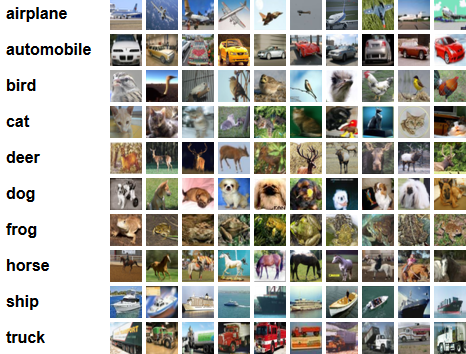
\includegraphics[width=0.8\textwidth]{../images/cifar.png}
	\caption{Example of images in the CIFAR-10 Dataset (source : \cite{cifar})}
	\label{cifar}
\end{figure}
\subsection{Convolutional Neural Networks}
Following the tutorials proposed on Keras website, it seems convolutional neural networks (CNN) are a good way to start for image classification.

It is based on the principle of scaling: some features are small and very specific, while other are big and generic. CNN uses convolution to reduce the image's dimension while taking every pixel into account. The weights give more or less importance to some scales and positions in the picture. 

Putting multiple layers of convolutions completely interconnected let the model finds high-level information on the picture. Usually, in between layers there is an activation function, whose task is to put values in a certain range. 

Multiple iterations of 3-4 convolution layers + activation layers, followed by a max pooling layer, and ending with some fully connected layers, is the suggested way for image classification in their tutorial.
\subsection{Implementation and results}
The model is constructed as follow : %change for picture of model
\begin{itemize}
	\item 2 repetitions of
	\begin{itemize}
		\item 3 repetitions of
		\begin{itemize}
			\item 1 convolution layer
			\item 1 activation layer (RELU)
		\end{itemize}
		\item 1 Max pooling layer
	\end{itemize}
	\item 2 fully connected layers	
\end{itemize}
It obtains around 75\% of accuracy for classification. 
\section{Prototype 1}
This prototype will determine if it's possible to generate sound from an image. It's goal is to be able to find the sound wave of a simple sine groove.
\subsection{SOTA machine learning models}
Over the years, multiple types of layers and neural networks were invented, each for a specific task. In this project, the goal is to generate precisely a sound wave from a groove image. It needs to be able to find the amplitude of the sound at a certain point on the groove. The amplitude is given by the perpendicular velocity of the needle when following the groove, meaning it's not the absolute position that is important, but the change of position.

Machine learning models generally try to find a solution for two types of problems : classification and regression.

Classification can be done while knowing what classes are possible, or just trying to cluster inputs together. If used with images, they are usually small (28x28 to 128x128).

Regression is the search of a continuous value given time based data points. It is usually used to predict future values.

For classification, our problem (finding the amplitude at a given moment) could be seen as classifying small groups of groove lines into an amplitude, since they are discrete (encoded in 32 bits maximum, ~4 billions classes). Reducing the encoding size would make it easier for a model, but quality would be lost.

For regression, the groove and sound could be seen as time series, and the goal would be to predict amplitude values.

Also, the problem can be seen as an interpolation one : given clean needle positions, what is the best curve to connect them ? Once determined, taking the derivative would give the sound wave.

If it is not possible to generate sound from images, other approaches can be taken (see Risks)

Here is a list of models, their application, and their relevance to our problem:
\begin{description}
	\item[Convolutional Neural Network - CNN] Can find detailed and general information on a picture, used for classification. Outputs a vector of class probabilities. This can be used for ML4NR by treating the output vector as a list of amplitudes in playing order.
	\item[Auto-encoder] Can remove noise by first finding the feature of the data while reducing it (encoding), and then expanding the feature to recreate the data (decoding). Used for image denoising, and interpolation. It can be used for this project.
	\item[Generative Adversarial Network - GAN] Composed of two parts competing against each other : one part tries to generate realistic data while the other tries to detect real and generated data. Used for dataset generation when real data is hard to obtain. Can be used for denoising. May apply in this project.
	\item[Residual Network - ResNet] Very deep network of convolutional layers (up to 150). The idea is to connect the input of a layer to the next layer, so they can learn by seeing processed and unprocessed data. Used for classification. Can be used here.
	\item[Recurrent Neural Network - RNN] Simple neural network, but the output of a layer is fed back to a previous layer. This allows it to learn from past values, and is good for time series. Used for regression. Can be used here.
	\item[Long Short-Term Memory - LSTM] Same idea as recurrent neural networks, it uses previous feature values to find the present output. The difference is the possibility to have as many previous data as needed. A special neuron is responsible for telling when a previous feature value is still relevant or not. Very good for time series, can be applied here.   
\end{description}
By tweaking the problem, all those models could be used. It is complicated to see what would be best, as no similar project were found. For this prototype, the first try is with a CNN model, like the one used in prototype 0. The second try is with a LSTM model.

\subsection{Risks}
If the model is really bad at finding the correct sound from the image, other methods could be used :
\begin{itemize}
\item Cleaning the image of its noise with an auto-encoder.
\item Finding the needle positions at successive time steps, and using the derivative to obtain the amplitude
\item Cleaning the generated audio of its noise
\end{itemize}

\subsection{Weaver plugins}
Weaver consists of more than 150 plugins, each doing a specific process. They are divided into categories : Load, Image, Track, Process, Save, Other.

All plugins inherit from the AbstractPlugin class, containing data useful to most of plugins. They are chained automatically when placed in the pipeline. 
\subsection{Dataset generation plugin}
A machine learning dataset needs to be as diverse as possible, in order to avoid over-fitting. A plugin able to generate a random dataset would be ideal.

Following the example pipeline for simple sine grooves given by Mr. Cornell %add in appendix
, a new plugin is implemented with these ideas in mind:
\begin{itemize}
	\item The images should be random in an acceptable range.
	\item It should be possible to generate systematically all combinations if desired.
	\item The dataset size can become quite big, an estimation of the size would be useful.
\end{itemize}

All sine groove parameters can be randomized. The most intuitive way to do it is to take minimum, maximum and step for each parameter. Setting minimum = maximum will generate only this value for this parameter.

\begin{figure}
	\centering
	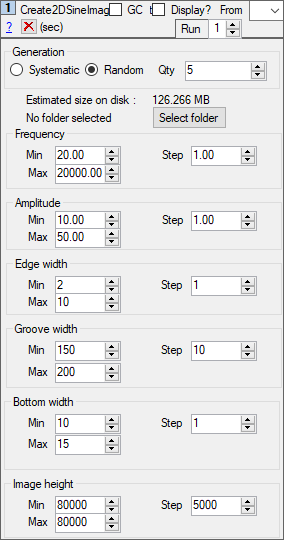
\includegraphics[width=0.5\textwidth]{../images/datasetplugin.png}
	\caption{Dataset generation plugin interface}
	\label{dsplugin}
\end{figure}

The file name contains the values used for each parameter. Then are encoded as the parameter's first letter and the value. Ex :

f1875\_a10\_e3\_b12\_g160\_h80000.tif

Using Weaver loop plugin, the corresponding sound of each image is generated.
\subsection{Dataset}
Here is what a generated groove looks like :
\begin{figure}
	\centering
	
\includegraphics[width=0.5\textwidth]{../images/example_groove.png}
	\caption{Generated groove, frequency=2760}
	\label{gengroove}
\end{figure}
The first idea is to generate randomized grooves so model inputs are as diverse as possible. However, the audio file generated from a random groove can sometimes be wrong. The algorithm used by Weaver plugins needs initial values close to the actual ones, and it's quite complicated with a random dataset. Furthermore, even the "correct" audio files contain some high frequency noise, due to the algorithm imperfection. We decide to generate the audio data from the code and not Weaver for this prototype.

The groove and image properties are fixed, for an easier manipulation of data for training. Only the frequency is randomized.
\begin{table}
	\begin{tabular}{|r|l|lll}
		\cline{1-2}
		Width        & 204        &  &  &  \\ \cline{1-2}
		Height       & 80'000     &  &  &  \\ \cline{1-2}
		Frequency    & 20 - 5'000 &  &  &  \\ \cline{1-2}
		Amplitude    & 10         &  &  &  \\ \cline{1-2}
		Edge width   & 3          &  &  &  \\ \cline{1-2}
		Groove width & 160        &  &  &  \\ \cline{1-2}
		Bottom width & 12         &  &  &  \\ \cline{1-2}
	\end{tabular}
\end{table}

In order to keep some space, we generate around 100 images.

So ideally, the input is a 204 x 80'000 8-bits image, and the output is a 104KHz 16-bits/channel stereo wave file.
\subsection{Model implementation}
\subsubsection{Version 1}
The first intuition is to use what we already know from prototype 0: the CNN layer.

The input is a 80'000 by 204 8-bits gray-scale groove image, and the goal is to find the WAV data of 80'000 samplings.
The audio file has two channels, even if most of the time they have the same value. Each channel is encoded in 16-bits. We only search for one channel and copy it for the second.

The first layer has to accept one groove image as input, as they are too heavy to all be loaded in memory. For each epoch, we loop through all images, feeding them one at a time to the model for fitting. The model is saved every epoch, because Google Colab, used for the implementations of this project, makes sessions expire after a fixed time.

\begin{figure}
	\centering
	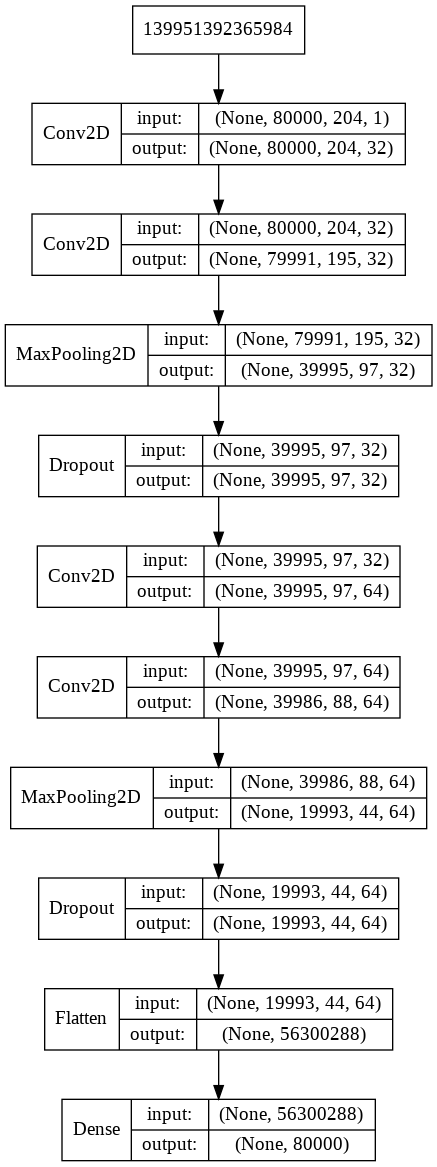
\includegraphics[width=0.5\textwidth]{../images/model_v1.png}
	\caption{Architecture of the convolutional network}
	\label{archiv1}
\end{figure}

\begin{figure}
	\centering
	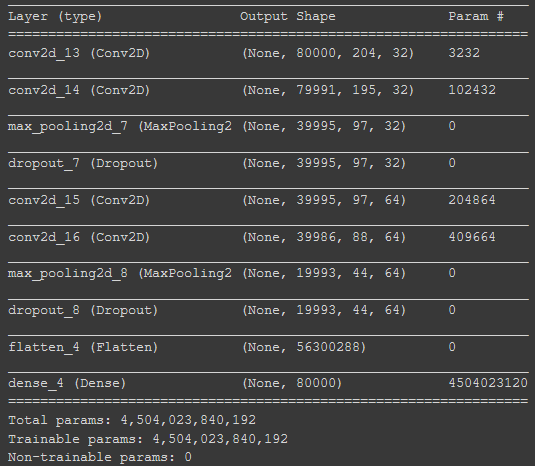
\includegraphics[width=0.7\textwidth]{../images/model_v1_params.png}
	\caption{Parameters count of the model}
	\label{paramv1}
\end{figure}

The convolutions kernel are 10x10 because 10 rows of data should help find the amplitude at a certain point, and 10 columns cover the groove edge. The output size of 32 is what is typically used in examples. Padding keeps the image at the same size.

A good optimizer is ADAM, who uses gradient descent. All parameters are left with default values. Mean square error (MSE) seems to be a perfect loss function for our problem, as the further we are from the ground-truth, the worse it is. Mean absolute error (MAE) can also provide insight on the results.

\subsubsection{Version 1 results}
After training for 10 epochs over 94 images, the best results are obtained by images whose audio contains a lot of 0. Their loss function score is however still horrible : in the order of 10'000s to 100'000s for MSE, 1000s for MAE. Images whose sounds have a lot of non-zero score in the order of 10'000'000s for MSE, and 10'000s for MAE.

Seeing that the loss scores increases over time, we know there is a problem with our parameters and/or inputs. 

Since it is a first shot at this problem through intuition, we decided to abandon this method and to search a better model.
\subsubsection{Version 2}
The first version being unsuccessful, we searched further in the current SOTA for regression problem linked to time series. A neural network that stood out was Long Short-Term Memory (LSTM).

LSTM are composed of neurons able to retain information from previous steps. They use them to predict values, but if an input from a previous step is no longer useful, it's able to forget it.

In order to use it with Keras, the inputs needs to be reshaped in three dimensions. The first is blocks of multiple rows. The second is the rows of features for one prediction, also called time steps. The third is the features.


Since it already is a full Neural Network (it generates a node for each feature at each time step), we decided to use only one of them for now. It will take one block of rows as input at a time, and output the amplitude for both channel at that time step.

\begin{figure}
	\centering
	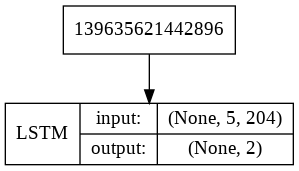
\includegraphics[width=0.5\textwidth]{../images/model_v2.png}
	\caption{Architecture of the LSTM network}
	\label{archiv2}
\end{figure}

\begin{figure}
	\centering
	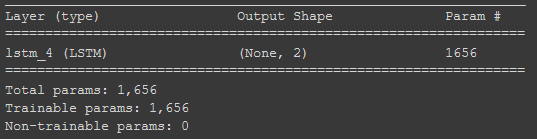
\includegraphics[width=0.7\textwidth]{../images/model_v2_params.png}
	\caption{Parameters count of the model}
	\label{paramv2}
\end{figure}

This model takes a 5 x 204 image as input, and gives 1 x 2 as output (the amplitude for both channels).

For the loss function and optimizer, we will keep the same as version 1.

\subsubsection{Version 2 - results}
After training for 10 epochs over 94 images, the results are in the same range as version 1. It seems the problem comes from the learning rate and the features, rather than the model itself.

\subsubsection{Version 3}
With version 2 results, we now know that the features are bad when used directly.

Following the advice of Mr. Hennebert, we normalize the inputs and target to obtain a nicer range. Each pixel of the groove image is normalized between 0 and 1. Each audio amplitude goal is normalized between -1 and 1.

Furthermore we use the CNN again, as it is easier to understand and fine tune. However, the input will have the same shape as in version 2 : a few rows of all pixels as input, and the amplitude of as output. Since the sound should be in mono, only one output value is needed.

\begin{figure}
	\centering
	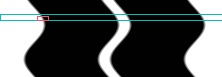
\includegraphics[width=0.8\textwidth]{../images/input.jpg}
	\caption{Window used to predict the amplitude}
	\label{input_v3}
\end{figure}

The blue rectangle is an example of input given to the model. The red rectangle is an example of convolutional kernel.

\begin{figure}
	\centering
	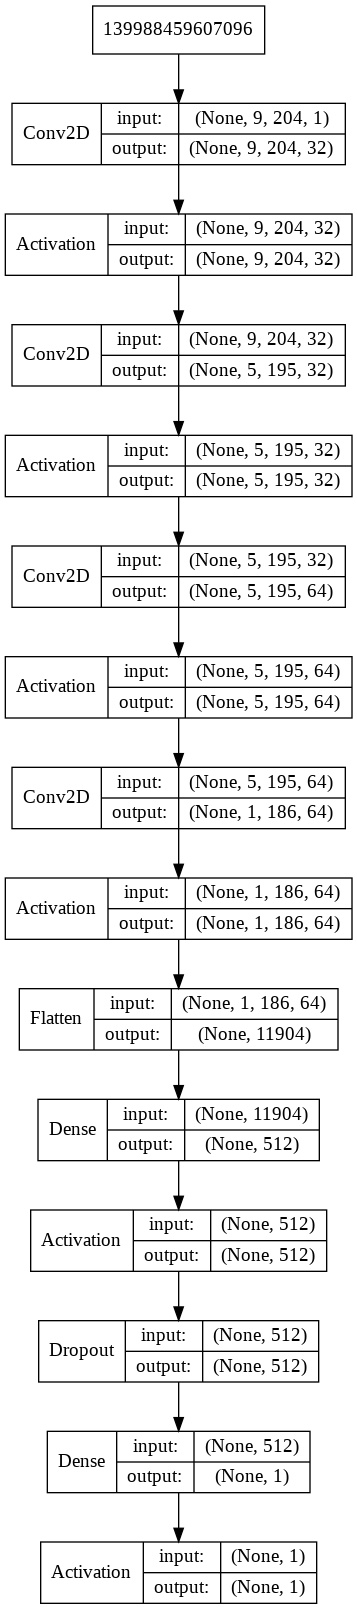
\includegraphics[width=0.3\textwidth]{../images/model_v3.png}
	\caption{Architecture of the CNN with window}
	\label{archiv3}
\end{figure}

\begin{figure}
	\centering
	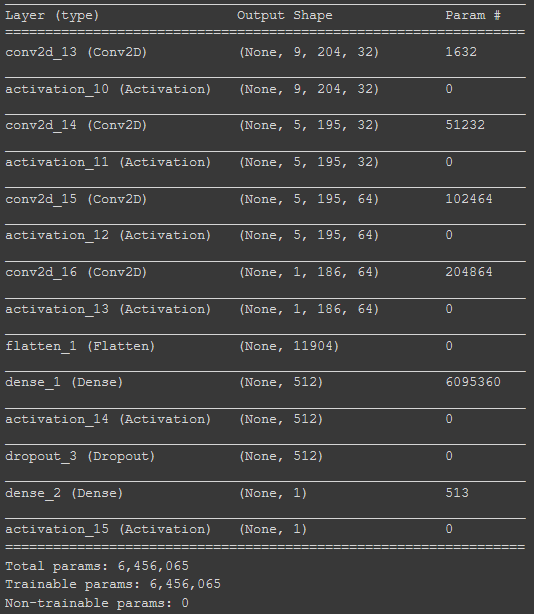
\includegraphics[width=0.7\textwidth]{../images/model_v3_params.png}
	\caption{Parameters count of the model}
	\label{paramv3}
\end{figure}

Each image is split into overlapping blocks of 9 rows and 204 features. They are then fed to the model, in which each convolutional layer tries to find hidden features in 5x10 matrices. 

For the two previous versions there were no activation layer, because the output wasn't bound. Here, since we are searching for an amplitude between -1 and 1, the tanh activation function seems reasonable.

The dropout layers make it harder to overfit.

The optimizer is also different : we use RMSprop, whose key advantage is the automatic adaptation of its learning rate. This avoids loss function triggering long jumps and divergence. The parameters used are learning\_rate=1e-4, decay=1e-6.

For validation, 15\% of the blocks of one image are taken out of training, and then used for scoring. Furthermore, after 25 images, a real sound generation is made from unseen images and saved (no scoring). This allows us to hear the results rather than comparing numbers.

\subsubsection{Version 3 - results}
This model seemed to have good results from the beginning, so everything was put in place to record the training : MSE and MAE scores for train and test images, weights saving, audio file registering.

Here are the MSE and MAE scores :

\begin{figure}
	\centering
	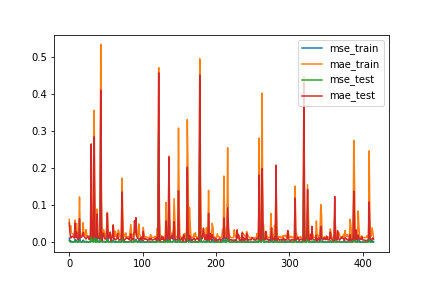
\includegraphics[width=0.8\textwidth]{../images/res_plot_v4.png}
	\caption{MSE and MAE for train and test scores}
	\label{scoresv3}
\end{figure}

We can see spikes. Those corresponds to low frequency grooves, where the lateral movement is really slow. We can see why the model has a hard time with them.

\begin{figure}
	\centering
	
\includegraphics[width=0.3\textwidth]{../images/low_freq.png}
	\caption{Groove of frequency 25}
	\label{lowfreq}
\end{figure}

A prediction of a low frequency groove has less amplitude, but the frequency itself seems to be correct.

\begin{figure}
	\centering
	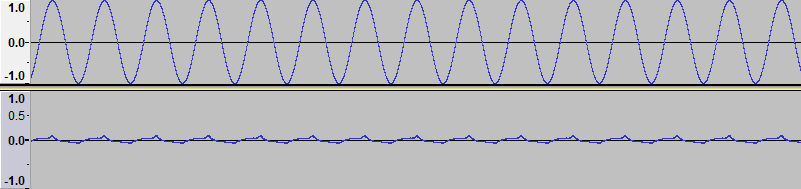
\includegraphics[width=1.0\textwidth]{../images/pred_60.png}
	\caption{Top : perfect sine wave of 60Hz / Bottom : predicted wave from groove}
	\label{pred60}
\end{figure}

Expanding the range after the generation could make it better.

As the frequency increases, the prediction is more spot on, and the audio sounds closer to the truth. 

\begin{figure}
	\centering
	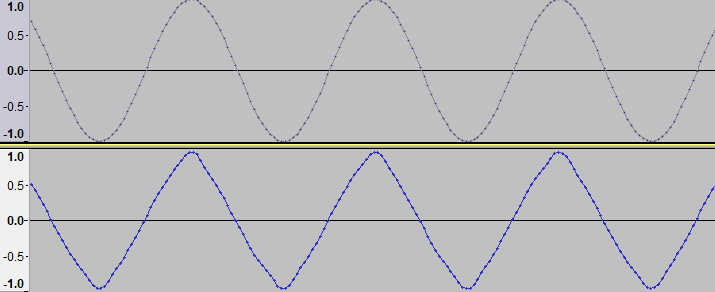
\includegraphics[width=1.0\textwidth]{../images/pred_2175.png}
	\caption{Top : perfect sine wave of 2175Hz / Bottom : predicted wave from groove}
	\label{pred2175}
\end{figure}

It is however very sharp, and analyzing the spectrum shows that a lot of higher frequencies are involved (mostly harmonics of our desired frequency).

\begin{figure}
	\centering
	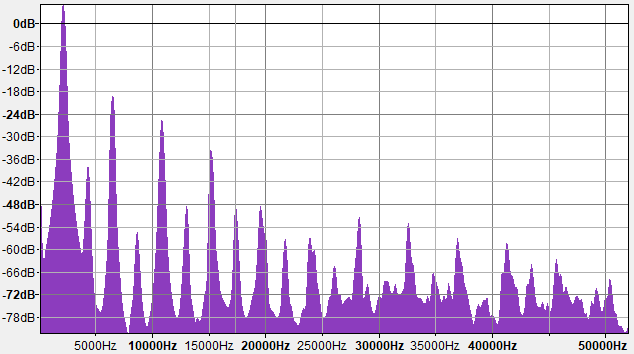
\includegraphics[width=0.8\textwidth]{../images/spectrometer_2175_v4.png}
	\caption{Spectrum of the generated audio for a 2175Hz groove}
	\label{spectrum2175}
\end{figure}

\subsubsection{Version 4}
In order to improve our results, fine-tuning all hyper-parameters is necessary. The success or failure of neural networks depends on it, as a bad combination could make the model and results diverge instead of converging.

The hyper-parameters of our model are :
\begin{description}
	\item[Batch size] Number of blocks given to train the network before updating the weights. Mainly depends on the memory available
	\item[Time steps] Number of rows of the sliding window. Too few and it will be hard to differentiate slopes of the groove. Too many and the model will take a long time to find what is useful.
	\item[Predictions] Number of amplitude points to find in one block. There may be a link between following amplitudes that the model can use to be more accurate.
	\item[Convolution filter shape] Convolution kernel size. Small filters can find smaller features, big ones can detect more general elements. Generally 3x3 in CNN.
	\item[Max pooling filter shape] Size of the kernel in which we keep only the maximum. Generally 2x2 in CNN.
	\item[Dropout rate] Proportion of neuron connections randomly cut to avoid over-fitting and accelerate learning time.
	\item[Activation function] Function that will collapse values on a certain range. \texttt{tanh} gives values between -1 and 1, \texttt{ReLu} between 0 and infinity.
	\item[Optimizer] Algorithm used to update the network weights. There exists a lot of them, with different properties and applications. Most of them need a learning rate and a decay rate.
	\item[Learning rate] Strength of the weight updates when searching the minimum loss. Too high and the values could diverge, too low and the learning will take a long time to find the minimum. 
	\item[Decay rate] Reduction of learning rate at every step, so it is less likely to diverge.
	\item[Loss function] Value calculated between predicted value and goal. This value is what the optimizer tries to minimize.
\end{description}

This makes a lot of parameters, and testing all possible combinations is impossible. Some of them seem to be more linked than others, and using intuition, are grouped like that :
\begin{enumerate}
	\item Time steps, predictions, and convolutional filter shape
	\item Max pooling shape and dropout
	\item Optimizer, learning rate, and decay rate
\end{enumerate}
Batch size can be fixed, as it should not have too much of an influence (32 is generally used). Loss function can also be fixed. For regression problem. a mean square error seems perfect.

Since the dataset is not noisy like the actual grooves, some of the parameters found here may not be ideal later. For this reason, the models are not trained for too long. One pass over all images should be enough to find the good combinations.

The input dataset is 78 images, each of them decomposed in up to 79'996 blocks using a sliding window. 15\% of them are taken away for validation, resulting in up to more than 5'300'000 blocks for training one epoch. The model trains on each block individually to find a certain number of predictions per block. This dataset should be big enough to have interesting results after one pass only.

In table \ref{hp1}, values considered for the first group of hyper-parameters can be found.
\begin{table}[H]
	\begin{tabular}{|r|l|l|l|l}
		\cline{1-4}
		Hyper-parameter				& Min	& Max 					& Step 	& \\ \cline{1-4}
		Time steps  				& 5    	& 9   					& 2    	& \\ \cline{1-4}
		Predictions 				& 1    	& Time steps  			& 2 	& \\ \cline{1-4}
		Convolution filter height  	& 3 	& Time steps / 2 + 0.5 	& 2 	& \\ \cline{1-4}
		Convolution filter width  	& 3 	& 9 					& 2 	& \\ \cline{1-4}
		
	\end{tabular}
	\caption{Range of values for hyper-parameters fine tuning}
	\label{hp1}
\end{table}

This already results in 104 possible combinations. In order not to lose too much time, only the 50 first combinations will be trained. If the best results are obtained with parameters values close to those that aren't trained yet, the remaining combinations will also be trained. However, if the best models are the ones with small parameter values, there is probably no need to train models with bigger values.

The other hyper-parameters seem more dependent on whether the dataset is noised or not, so they will be fine-tuned in prototype 2. 
\subsubsection{Version 4 results}
For result evaluation, every model tries to predict the audio wave of the 18 test images. The mean square errors of each prediction are averaged together to obtain the global test result.

The best results, after training over 78 images of grooves with variable frequency, are obtained by the first model tested (results of best three models in figure \ref{resp1v4}).

\begin{figure}
	\centering
	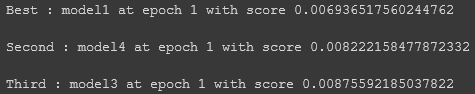
\includegraphics[width=0.8\textwidth]{../images/resp1v4.png}
	\caption{Top three results obtained by different combinations}
	\label{resp1v4}
\end{figure}

All three models have small hyper-parameters values : all have time steps = 5, predictions = 1, and convolution filter height = 3. The only difference between them is convolution filter width, which is in order 3, 7 and 9.

All the other results can be found in the annex. TODO add ref

It can be assumed that there is no need to train models with bigger parameter values.

In table \ref{hpm1}, you can find the values used by the best model.

\begin{table}
	\begin{tabular}{|r|l|lll}
		\cline{1-2}
		Time steps        & 5        &  &  &  \\ \cline{1-2}
		Predictions       & 1     &  &  &  \\ \cline{1-2}
		Convolution filter    & 3x3 &  &  &  \\ \cline{1-2}
		Max pooling filter    & 2x2        &  &  &  \\ \cline{1-2}
		Dropout rate   & 0.25 (firsts) and 0.5 (last)          &  &  &  \\ \cline{1-2}
		Activation function & ReLu (firsts) and tanh (last)        &  &  &  \\ \cline{1-2}
		Optimizer & RMSprop         &  &  &  \\ \cline{1-2}
		Learning rate & 1e-4         &  &  &  \\ \cline{1-2}
		Decay rate & 1e-6         &  &  &  \\ \cline{1-2}
	\end{tabular}
	\caption{Hyper-parameters used for best results}
	\label{hpm1}
\end{table}

The model architecture can be found in the annex. TODO add ref

For reference, the goal and predicted signals can be seen in figure \ref{predm1}.
\begin{figure}
	\centering
	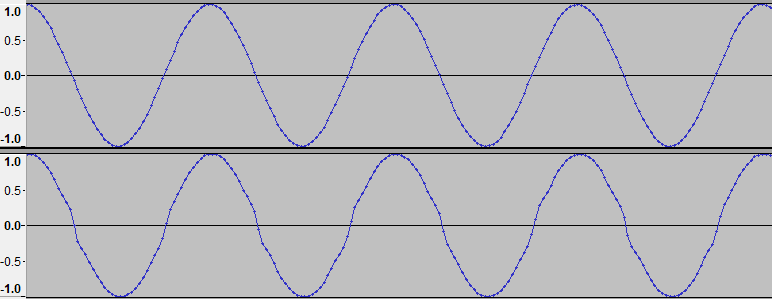
\includegraphics[width=0.8\textwidth]{../images/predm1.png}
	\caption{Top : goal signal of 2175Hz. Bottom : predicted signal}
	\label{predm1}
\end{figure}
Compared to the previous prediction of the same groove (figure \ref{pred2175}), this one looks better, especially at the peaks.

The spectrum (figure \ref{spectrumm1}) also shows a big difference between the main frequency and the overtones, indicating a reduced background noise
\begin{figure}
	\centering
	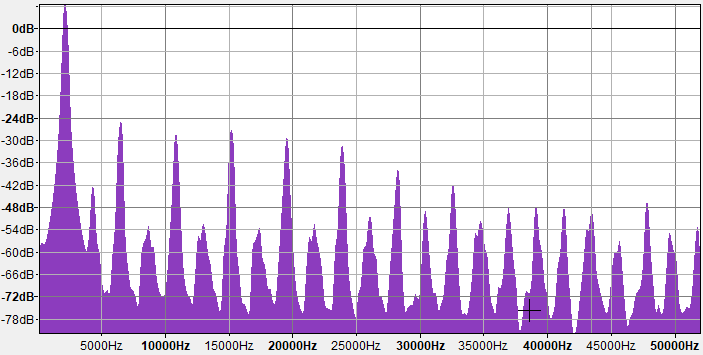
\includegraphics[width=0.8\textwidth]{../images/spectrum_m1.png}
	\caption{Spectrum of the predicted audio wave}
	\label{spectrumm1}
\end{figure}
\section{Prototype 2}
In this prototype, the goal is to train a model on noisy images of single frequency grooves and make it predict a perfect sine wave.
\subsection{Noisy groove images}
As can be seen in figure \ref{vayabis}, the actual disc images are noisy. 
\begin{figure}
	\centering
	\includegraphics[width=0.4\textwidth]{../images/Vaya-52212c.png}
	\caption{One image of the shellac disc of Vaya Con Dios, by Les Paul and Mary Ford (source : lab's collection)}
	\label{vayabis}
\end{figure}
That noise can be decomposed in different type of noise :
\begin{itemize}
	\item A light Gaussian noise that gets heavier on the groove edges, caused by dust and texture.
	\item Thin scratches that are seen as black.
	\item Bigger damage that is also seen as black.
\end{itemize}
All those makes the task of finding the sound more difficult, it is therefore important to simulate them for model training.
\subsection{Artificially noised dataset}
Since a dataset of grooves and their output is already available, a simple program can be used to noise them and generate a new dataset. Those noised grooves should look as much as possible as the actual disc images.

The Gaussian noise can be added easily on the perfect groove image. The black part should stay as dark as possible, and the white part should have visible deterioration. Knowing that the pixel values are between 0 and 255, a Gaussian noise of average -100 and standard deviation of 50 is clearly visible on the white parts and not so much on the black ones.

For the scratches, thin long black rectangles are generated randomly and placed randomly across the image.

For the big damage, the same is done with bigger black rectangles, but not as many as scratches.

The result of artificial noising can be seen in figure \ref{cleannoisy}.

\begin{figure}
	\centering
	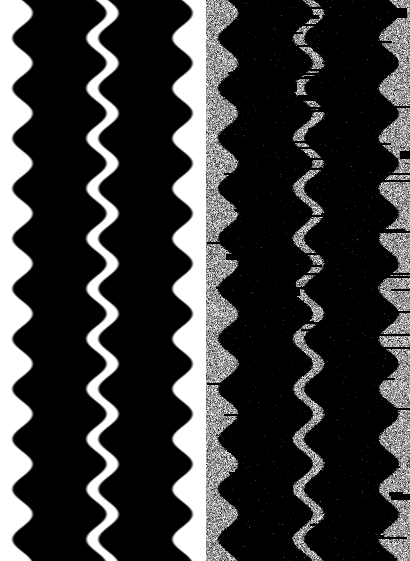
\includegraphics[width=0.5\textwidth]{../images/cleannoisy.png}
	\caption{Left : clean groove of 2075 Hz. Right : same groove artificially noised}
	\label{cleannoisy}
\end{figure}

\subsection{Version 1}
In this version, the dataset is the same as for prototype 1 (78 images for training, 18 for testing). All the images are noised once and written in static memory, so the training and testing images are the same for all models.

The goal is to obtain a good prediction of the sound wave of a noisy groove image. In order to do that, further fine tuning is necessary.
Instead of trying every combination like before, parameter values are tuned through trial and error.
\subsubsection{Implementation}
The first model trained is the one that obtained the best results in prototype 1.

Then, fine tuning over the learning and decay rate are tried. In the first model RMSprop is used, and the values are learning = 1e-4, decay = 1e-6. However, Keras documentation suggest using default values, which are learning = 1e-3 and decay = 0. We can also try to make the decay bigger to see how it affects learning.

Seeing the noised images, it seems a bigger sliding window could help find amplitude more easily when the groove edge is damaged. Big jumps in values make it faster to see if it's relevant or not to change it, so the network is tested with window height (time steps) of 5, 9, and 15.

Each model is trained over a varying number of epochs, depending on the occasional crash of the connection and the time taken.
\subsubsection{Results}
First come the results between the different learning and decay rates. Figure \ref{resp2v1lr} shows the results of the three best model and epoch.
\begin{figure}
	\centering
	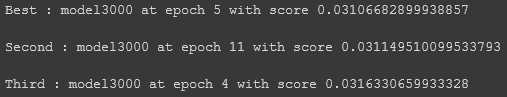
\includegraphics[width=0.8\textwidth]{../images/resp2v1lr.png}
	\caption{Top three results among all epochs and models where learning and decay rates are tuned}
	\label{resp2v1lr}
\end{figure}

The model using learning rate = 1e-4 and decay rate = 1e-6 obtains the three best results. However, the results don't seem to improve over time. It can be a sign of bad values or even bad optimizer. 

Next, using the default values of the RMSprop optimizer, the window height parameter is played with. Again, figure \ref{resp2v1ts} shows the results of the three best model and epoch.
\begin{figure}
	\centering
	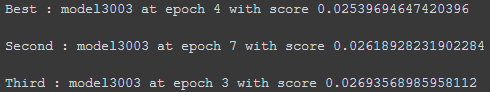
\includegraphics[width=0.8\textwidth]{../images/resp2v1ts.png}
	\caption{Top three results among all epochs and models where sliding window size is tuned}
	\label{resp2v1ts}
\end{figure}

This time, the results are a bit better. The best model is the one using a window height of 15 pixels. Our intuition proved to be right.
\subsection{Version 2}
In this version, a new dataset is used : groove images are now lightly randomized (groove width, edge width, bottom width), and they are noised on the fly during training. The test dataset is noised once, written in memory, and used for every model so comparisons make sense.

The training dataset contains 170 images, the test 30 images. 15\% of image blocks are used for validation. This makes training for one epoch quite long (around 3 hours with our current environment). Furthermore, a good result over the test set could be obtained in the middle of an epoch. With these two arguments in mind, a modification was made to th program : it is now possible to divide the training dataset and to test results after each smaller division. This also allows to resume training in case of crash.

In the previous version, the optimizer didn't seem to work correctly even with different values. In this version, other optimizers are tested : Adagrad and Adam.
\subsubsection{Implementation}
First, the best hyper-parameters previously found are used to train on the dynamic dataset. The same data is never seen twice, so the model should be more robust.

Then, optimizers Adagrad and Adam are tested with their default values.

The training dataset is divided in 10 smaller parts, and after each of them the model is tested.
\subsubsection{Results}
The model combining the best hyper-parameters and RMSprop optimizer trained over 6 epochs. The best results are obtained on epoch 1, showing that there is indeed a problem with the optimizer. However, it was used to make a prediction and see if the model can find the audio of a noised groove.

Figure \ref{groove1530} is the noisy groove used for test (never seen during training). Figure \ref{predm4000} is the perfect wave and the predicted one. Figure \ref{spectrum4000} is the spectrum of the predicted audio wave.
\begin{figure}
	\centering
	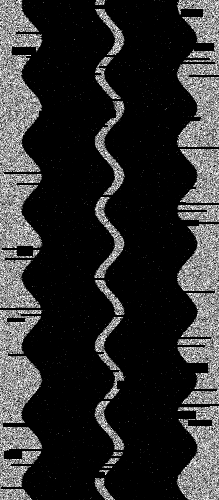
\includegraphics[width=0.4\textwidth]{../images/groove1530.png}
	\caption{Noisy 1530 Hz groove image used for testing}
	\label{groove1530}
\end{figure}
\begin{figure}
	\centering
	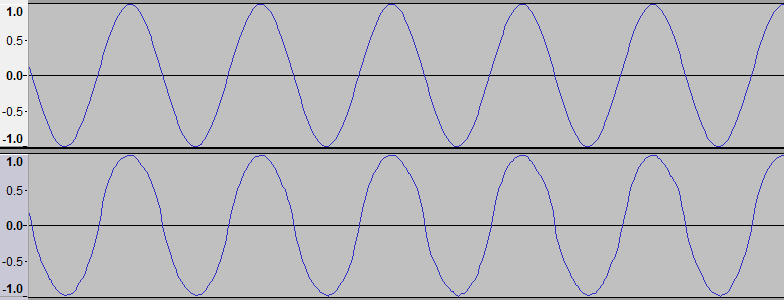
\includegraphics[width=0.8\textwidth]{../images/predm4000.png}
	\caption{Top : perfect 1530 Hz wave. Bottom : predicted wave from noisy groove image}
	\label{predm4000}
\end{figure}
\begin{figure}
	\centering
	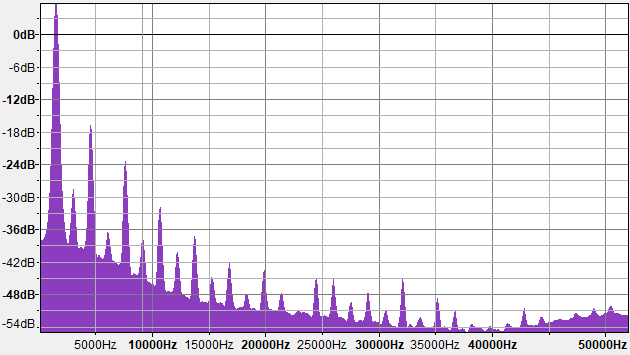
\includegraphics[width=0.8\textwidth]{../images/spectrum_m4000.png}
	\caption{Spectrum of the predicted 1530 Hz wave}
	\label{spectrum4000}
\end{figure}
The predicted wave looks thicker on the peaks. We can see that there are still overtones, however they quickly lose intensity. The predicted wave has some irregularities, but they are really small compared to the rest. It seems that even though it doesn't converge, this model is robust enough to predict a sound wave from a noisy image. TODO comparison with weaver output.

The next model to test has the same hyper-parameters except for the optimizer. It uses Adam with its default rates. The best test results are obtained at epoch 2.6. This epoch weights are used to make a prediction on the same groove as before. In figure \ref{pred4004} we can see the predicted sound wave on third position, the second being the prediction using RMSprop optimizer.
\begin{figure}
	\centering
	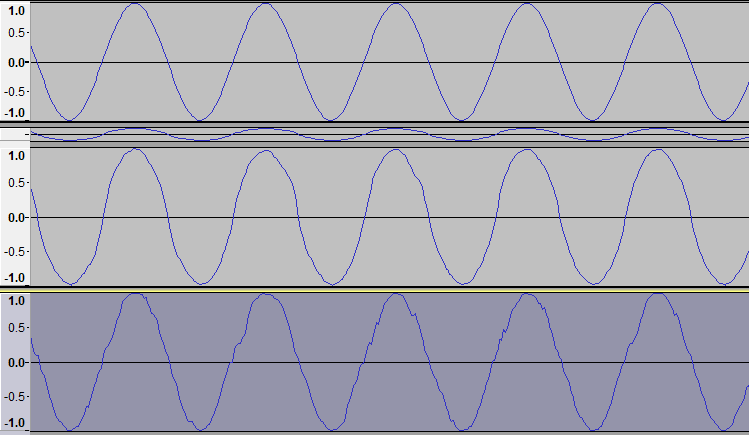
\includegraphics[width=0.8\textwidth]{../images/pred4004.png}
	\caption{Top : perfect 1530 Hz wave. Middle :  predicted wave from noisy groove image with RMSprop. Bottom : predicted wave from noisy groove image with Adam}
	\label{predm4004}
\end{figure}
We can see that the general shape is more similar to the perfect wave, however there are sharper errors. The spectrum (figure \ref{spectrum4004}) also shows overtones with less amplitude. It is a better result altogether.
\begin{figure}
	\centering
	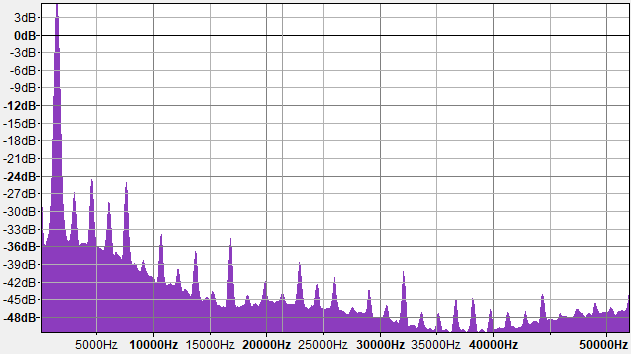
\includegraphics[width=0.8\textwidth]{../images/spectrum_m4004.png}
	\caption{Spectrum of the predicted audio wave}
	\label{spectrum4004}
\end{figure}
\section{Prototype 3 and 4}
In this prototype, the goal is to train a model on the real disc groove images, and to obtain a good prediction. The first attempt is a direct transfer learning from prototype 2. If it is not satisfying, a new model is trained
\subsection{Dataset formatting}
Weaver tracking -> center of sliding window
Writting lots of small images in memory
Original tape recording -> audio wave goal
\subsection{Implementation}
\subsection{Results}

\section{Conclusion}
\subsection{Personal opinion}
\subsection{Future work}

\bibliographystyle{unsrt}
\bibliography{cdc}
\includepdf[pages={3}]{planV1.pdf}
\end{document}